\documentclass[12pt]{report}
\usepackage[utf8]{inputenc}
\usepackage[russian]{babel}
%\usepackage[14pt]{extsizes}
\usepackage{listings}
\usepackage{graphicx}
\usepackage{amsmath,amsfonts,amssymb,amsthm,mathtools} 
\usepackage{pgfplots}
\usepackage{filecontents}
\usepackage{float}
\usepackage{indentfirst}
\usepackage{eucal}
\usepackage{enumitem}
%s\documentclass[openany]{book}
\frenchspacing

\usepackage{indentfirst} % Красная строка


\usetikzlibrary{datavisualization}
\usetikzlibrary{datavisualization.formats.functions}

\usepackage{amsmath}


% Для листинга кода:
\lstset{ %
language=c,                 % выбор языка для подсветки (здесь это С)
basicstyle=\small\sffamily, % размер и начертание шрифта для подсветки кода
numbers=left,               % где поставить нумерацию строк (слева\справа)
numberstyle=\tiny,           % размер шрифта для номеров строк
stepnumber=1,                   % размер шага между двумя номерами строк
numbersep=5pt,                % как далеко отстоят номера строк от подсвечиваемого кода
showspaces=false,            % показывать или нет пробелы специальными отступами
showstringspaces=false,      % показывать или нет пробелы в строках
showtabs=false,             % показывать или нет табуляцию в строках
frame=single,              % рисовать рамку вокруг кода
tabsize=2,                 % размер табуляции по умолчанию равен 2 пробелам
captionpos=t,              % позиция заголовка вверху [t] или внизу [b] 
breaklines=true,           % автоматически переносить строки (да\нет)
breakatwhitespace=false, % переносить строки только если есть пробел
escapeinside={\#*}{*)}   % если нужно добавить комментарии в коде
}

\usepackage[left=2cm,right=2cm, top=2cm,bottom=2cm,bindingoffset=0cm]{geometry}
% Для измененных титулов глав:
\usepackage{titlesec, blindtext, color} % подключаем нужные пакеты
\definecolor{gray75}{gray}{0.75} % определяем цвет
\newcommand{\hsp}{\hspace{20pt}} % длина линии в 20pt
% titleformat определяет стиль
\titleformat{\chapter}[hang]{\Huge\bfseries}{\thechapter\hsp\textcolor{gray75}{|}\hsp}{0pt}{\Huge\bfseries}


% plot
\usepackage{pgfplots}
\usepackage{filecontents}
\usetikzlibrary{datavisualization}
\usetikzlibrary{datavisualization.formats.functions}

\begin{document}
%\def\chaptername{} % убирает "Глава"
\thispagestyle{empty}
\begin{titlepage}
	\noindent \begin{minipage}{0.15\textwidth}
	
\includegraphics[width=\linewidth]{img/b_logo}
	\end{minipage}
	\noindent\begin{minipage}{0.9\textwidth}\centering
		\textbf{Министерство науки и высшего образования Российской Федерации}\\
		\textbf{Федеральное государственное бюджетное образовательное учреждение высшего образования}\\
		\textbf{~~~«Московский государственный технический университет имени Н.Э.~Баумана}\\
		\textbf{(национальный исследовательский университет)»}\\
		\textbf{(МГТУ им. Н.Э.~Баумана)}
	\end{minipage}
	
	\noindent\rule{18cm}{3pt}
	\newline\newline
	\noindent ФАКУЛЬТЕТ $\underline{\text{«Информатика и системы управления»}}$ \newline\newline
	\noindent КАФЕДРА $\underline{\text{«Программное обеспечение ЭВМ и информационные технологии»}}$\newline\newline\newline\newline\newline
	
	\begin{center}
		\noindent\begin{minipage}{1.3\textwidth}\centering
			\Large\textbf{  Отчет по лабораторной работе №5}\newline
			\textbf{по дисциплине "Операционные системы"}\newline\newline
		\end{minipage}
	\end{center}
	
	\noindent\textbf{Тема} $\underline{\text{Взаимодействие параллельных процессов~~~~}}$\newline\newline
	\noindent\textbf{Студент} $\underline{\text{Романов А.В.~~~~~~~~~~~~~~~~~~~~~~~~~~~~~~~~~~~~~~}}$\newline\newline
	\noindent\textbf{Группа} $\underline{\text{ИУ7-53Б~~~~~~~~~~~~~~~~~~~~~~~~~~~~~~~~~~~~~~~~~~~~~~}}$\newline\newline
	\noindent\textbf{Оценка (баллы)} $\underline{\text{~~~~~~~~~~~~~~~~~~~~~~~~~~~~~~~~~~~~~~~~~~~~~}}$\newline\newline
	\noindent\textbf{Преподаватели} $\underline{\text{Рязанова Н.Ю.~~~~~~~~~~~~~~~~~~~~~~~~~~}}$\newline\newline\newline
	
	\begin{center}
		\vfill
		Москва~---~\the\year
		~г.
	\end{center}
\end{titlepage}

\chapter{Задача <<Производство-потребление>>}

\section{Демонстрация работы программы}

\begin{figure}[H]
	\centering
	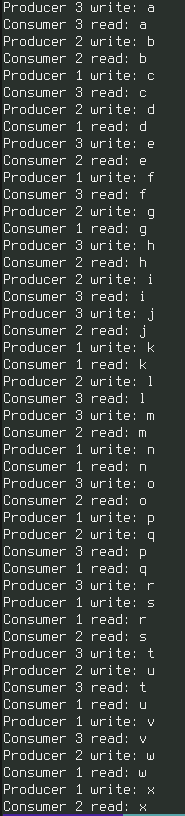
\includegraphics[scale=0.55]{img/prod-cons-01.png}
	\caption{Демонстрация работы программы <<Производство-потребление>>. Задержка потребителя: от 1 до 4, задержка производителя: от 1 до 4}
	\label{fig:task01-01}
\end{figure}

\begin{figure}[H]
	\centering
	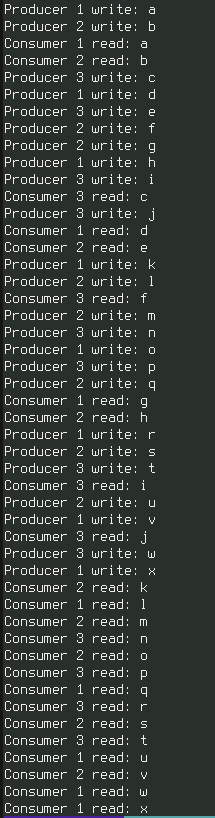
\includegraphics[scale=0.75]{img/prod-cons-02.png}
	\caption{Демонстрация работы программы <<Производство-потребление>>. Задержка потребителя: от 1 до 9, задержка производителя: от 1 до 4}
	\label{fig:task01-02}
\end{figure}

\begin{figure}[H]
	\centering
	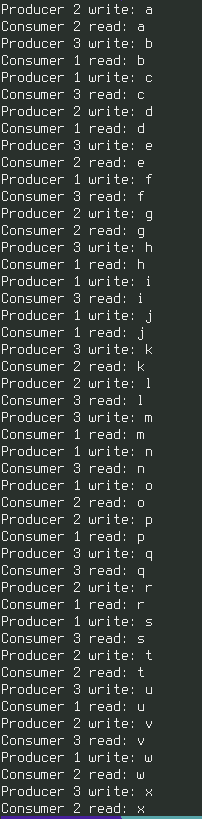
\includegraphics[scale=0.75]{img/prod-cons-03.png}
	\caption{Демонстрация работы программы <<Производство-потребление>>. Задержка потребителя: от 1 до 4, задержка производителя: от 1 до 9}
	\label{fig:task01-03}
\end{figure}

\section{Листинги кода}

В листингах \ref{buffer} - \ref{main} представленны исходные коды решения задачи <<Производство-потребление>>.


\begin{lstlisting}[label=buffer,caption=Реализация очереди на основе циклического буффера,language=C]
#include "buffer.h"

int init_buffer(cbuffer_t *const buf) {
	if (!buf) {
		perror("Error while initializing buffer.\n");
		return BUF_ERR;
	}
	
	return OK;
}

int write_buffer(cbuffer_t *const buf, const char element) {
	if (!buf) {
		return BUF_ERR;
	}
	
	buf->buffer[buf->write_pos++] = element;
	buf->write_pos %= N;
	
	return OK;
}

int read_buffer(cbuffer_t *buf, char *const element) {
	if (!buf) {
		return BUF_ERR;
	}

	if (!element) {
		return BUF_ERR;
	}

	*element = buf->buffer[buf->read_pos++];
	buf->read_pos %= N;

	return OK;
}
\end{lstlisting}

\begin{lstlisting}[label=consumer,caption=Реализация <<потребителей>>,language=C]
#include "consumer.h"

struct sembuf CONS_LOCK[] = { 
	{ BUFF_FULL, -1, 0 }, 
	{ BIN_SEM, -1, 0 } 
};

struct sembuf CONS_RELEASE[] = { 
	{ BUFF_EMPTY, 1, 0 }, 
	{ BIN_SEM, 1, 0 } 
};

int consumer_run(cbuffer_t *const buf, const int sid, const int consid) {
	srand(time(NULL) + consid);
	
	if (!buf) {
		return BUF_ERR;
	}
	
	for (int i = 0; i < ITER_CNT; i++) {
		int sleep_time = rand() % CONS_TIME_RANGE + CONS_TIME_START;
		sleep(sleep_time);
	
		if (-1 == semop(sid, CONS_LOCK, SEM_SIZE)) {
		
		return CONS_LOCK_ERROR;
		}
		
		char symb;
		
		if (-1 == read_buffer(buf, &symb)) {
			return BUFF_READ_ERROR;
		}
		
		fprintf(stdout, "Consumer %d read: %c\n", consid + 1, symb);
		
		if (-1 == semop(sid, CONS_RELEASE, SEM_SIZE)) {
			return CONS_RELEASE_ERROR;
		}
	}
	
	return OK;
}
\end{lstlisting}

\begin{lstlisting}[label=producer,caption=Реализация <<производителей>>,language=C]
#include "producer.h"

struct sembuf PROD_LOCK[] = { 
	{ BUFF_EMPTY, -1, 0 }, 
	{ BIN_SEM, -1, 0 } 
};

struct sembuf PROD_RELEASE[] = { 
	{ BUFF_FULL, 1, 0 }, 
	{ BIN_SEM, 1, 0 } 
};

int producer_run(cbuffer_t *const buf, const int sid, const int prodid) {
	srand(time(NULL) + prodid);
	
	if (!buf) {
	return BUF_ERR;
	}
	
	for (size_t i = 0; i < ITER_CNT; i++) {
		int sleep_time = rand() % PROD_TIME_RANGE + PROD_TIME_START;
		sleep(sleep_time);
		
		if (-1 == semop(sid, PROD_LOCK, SEM_SIZE)) {
			return PROD_LOCK_ERROR;
		}
		
		const char symb = (buf->write_pos % 26) + 'a';
		if (-1 == write_buffer(buf, symb)) {
			return BUFF_WRITE_ERROR;
		}
		
		fprintf(stdout, "Producer %lu write: %c\n", prodid + 1, symb);
		
		if (-1 == semop(sid, PROD_RELEASE, SEM_SIZE)) {
			return PROD_RELEASE_ERROR;
		}
	}
	
	return OK;
}
\end{lstlisting}

\begin{lstlisting}[label=main,caption=Главный файл программы,language=C]
#include <stdio.h>
#include <sys/ipc.h>
#include <sys/shm.h>
#include <sys/stat.h>
#include <sys/sem.h> 
#include <unistd.h>
#include <wait.h>

#include "buffer.h"
#include "consumer.h"
#include "producer.h"

#define PROD_CNT 3
#define CONS_CNT 3

#define PERMISSIONS S_IRWXU | S_IRWXG | S_IRWXO
#define SHMAT_ERR_RET (void *)-1

#define SEM_CNT 3
#define BIN_SEM 0
#define BUFF_FULL 1
#define BUFF_EMPTY 2

#define FREE 1

#define SHMGET_ERROR 1
#define SHMAT_ERROR 2
#define FORK_ERROR 3
#define WAIT_ERROR 4
#define SHUTDOWN_ERROR 5
#define SEMGET_ERROR 12

int main() {
	setbuf(stdout, NULL);
	
	int fd = shmget(IPC_PRIVATE, sizeof(cbuffer_t), PERMISSIONS | IPC_CREAT);
	if (-1 == fd) {
		perror("Error while creating shared memory.\n");
		return SHMGET_ERROR;
	}
	
	cbuffer_t *buffer = shmat(fd, 0, 0);
	if (SHMAT_ERR_RET == buffer) {
		perror("Error while creating shmat.\n");
		return SHMAT_ERROR;
	}
	
	if (BUF_ERR == init_buffer(buffer)) {
		return BUF_ERR;
	}
	
	int sid = semget(IPC_PRIVATE, SEM_CNT, PERMISSIONS | IPC_CREAT);
	if (-1 == sid) {
		perror("Error while creating array of semaphores.\n");
		return SEMGET_ERROR;
	}
	
	semctl(sid, BIN_SEM, SETVAL, FREE);
	semctl(sid, BUFF_EMPTY, SETVAL, N);
	semctl(sid, BUFF_FULL, SETVAL, 0);
	
	for (size_t i = 0; i < PROD_CNT; i++) {
		int child_pid = fork();
		
		if (-1 == child_pid) {
			perror("Error while fork (producer).");
			return FORK_ERROR;
		} else if (0 == child_pid) {
			producer_run(buffer, sid, i);
			return OK;
		}
	}
	
	for (size_t i = 0; i < CONS_CNT; i++) {
		int child_pid = fork();
		
		if (-1 == child_pid) {
			perror("Error while fork (consumer).");
			return FORK_ERROR;
		} else if (0 == child_pid) {
			consumer_run(buffer, sid, i);
			return OK;
		}
	}
	
	for (size_t i = 0; i < PROD_CNT + CONS_CNT; i++) {
		int statval;
		
		if (-1 == wait(&statval)) {
			perror("Error with child process.\n");
			return WAIT_ERROR;
		}
		
		if (!WIFEXITED(statval)) {
			fprintf(stderr, "Children process %lu terminated abnormally.", i);
		}
	}
		
	if (-1 == shmdt((void *)buffer) || -1 == shmctl(fd, IPC_RMID, NULL) || -1 == semctl(sid, IPC_RMID, 0)) {
		perror("Error while shutdown.\n");
		return SHUTDOWN_ERROR;
	}
	
	return OK;
}
\end{lstlisting}

\chapter{Задача <<Читатели-писатели>>}

\section{Демонстрация работы программы}

\begin{figure}[H]
	\centering
	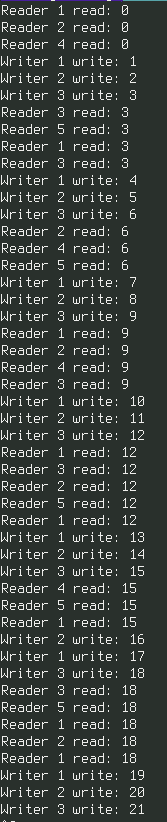
\includegraphics[scale=0.55]{img/read-write.png}
	\caption{Демонстрация работы программы <<Читатели-писатели>>.}
	\label{fig:task02}
\end{figure}

\section{Листинги кода}

В листингах \ref{buffer} - \ref{main} представленны исходные коды решения задачи <<Читатели-писатели>>.

\begin{lstlisting}[label=reader,caption=Реализация <<читателей>> и <<писателей>>,language=C]
#include "read_write.h"

struct sembuf READER_QUEUE[] = { 
	{ READ_QUEUE, 1, 0 }, 
	{ ACTIVE_WRITER, 0, 0 }, 
	{ WRITE_QUEUE, 0, 0 },
};

struct sembuf READER_LOCK[] = { 
	{ ACTIVE_READER, 1, 0 }, 
	{ READ_QUEUE, -1, 0 }, 
};

struct sembuf READER_RELEASE[] = { 
	{ ACTIVE_READER, -1, 0 }, 
};

struct sembuf WRITER_LOCK[] = {  
	{ ACTIVE_WRITER, 1, 0 }, 
	{ WRITE_QUEUE, -1, 0 },
};

struct sembuf WRITER_RELEASE[] = { 
	{ ACTIVE_WRITER, -1, 0 }, 
}; 

struct sembuf WRITER_QUEUE[] = { 
	{ WRITE_QUEUE, 1, 0 }, 
	{ ACTIVE_READER, 0, 0 }, 
	{ ACTIVE_WRITER, 0, 0 }, 
};

int start_read(int sid) {
	return semop(sid, READER_QUEUE, 3) != -1 && semop(sid, READER_LOCK, 2) != -1;
}

int stop_read(int sid) {
	return semop(sid, READER_RELEASE, 1) != -1;
}

int start_write(int sid) {
	return semop(sid, WRITER_QUEUE, 3) != -1 && semop(sid, WRITER_LOCK, 2) != -1;
}

int stop_write(int sid) {
	return semop(sid, WRITER_RELEASE, 1) != -1;
}

int reader_run(int *const shared_mem, const int sid, const int rid) {
	srand(time(NULL) + rid);
	
	if (!shared_mem) {
		return SHRDMEM_PTR_ERROR;
	}
	
	for (size_t i = 0; i < ITER_CNT; i++) {
		int sleep_time = rand() % TIME_RANGE + TIME_START;
		sleep(sleep_time);
		
		if (!start_read(sid)) {
			return READ_LOCK_ERROR;
		}
		
		int readed = *shared_mem;
		fprintf(stdout, "Reader %d read: %d\n", rid + 1, readed);
		
		if (!stop_read(sid)) {
			return READ_RELEASE_ERROR;
		}
	}

	return OK;
}

int writer_run(int *const shared_mem, const int sid, const int wid) {
	srand(time(NULL) + wid);
	
	if (!shared_mem) {
		return SHRDMEM_PTR_ERROR;
	}
	
	for (size_t i = 0; i < ITER_CNT; i++) {
		int sleep_time = rand() % TIME_RANGE + TIME_START;
		sleep(sleep_time);
		
		if (!start_write(sid)) {
			return WRITE_LOCK_ERROR;
		}
		
		int updated = ++(*shared_mem);
		fprintf(stdout, "Writer %d write: %d\n", wid + 1, updated);
		
		if (!stop_write(sid)) {
			return WRITE_RELEASE_ERROR;
		}
	}
	
	return OK;
}
\end{lstlisting}

\begin{lstlisting}[label=main-02,caption=Главный файл программы,language=C]
#include <stdio.h>
#include <sys/shm.h>
#include <sys/stat.h>
#include <unistd.h>
#include <sys/types.h>
#include <sys/ipc.h>
#include <sys/sem.h> 
#include <wait.h>

#include "read_write.h"

#define PERMISSIONS S_IRWXU | S_IRWXG | S_IRWXO
#define SHMAT_ERR_RET (void *)-1

#define READERS_CNT 5
#define WRITERS_CNT 3
#define SEM_CNT 4

#define OK 0
#define SHMGET_ERROR 1
#define SHMAT_ERROR 2
#define SEMGET_ERROR 3
#define FORK_ERROR 4
#define WAIT_ERROR 5
#define SHUTDOWN_ERROR 6

int main() {
	setbuf(stdout, NULL);
	
	int fd = shmget(IPC_PRIVATE, sizeof(int), PERMISSIONS | IPC_CREAT);
	if (-1 == fd) {
		perror("Error while creating shared memory.\n");
		return SHMGET_ERROR;
	}
	
	int *shared_mem_ptr = shmat(fd, 0, 0);
	if (SHMAT_ERR_RET == shared_mem_ptr) {
		perror("Error while creating shmat.\n");
		return SHMAT_ERROR;
	}
	
	int sid = semget(IPC_PRIVATE, SEM_CNT, PERMISSIONS | IPC_CREAT);
	if (-1 == sid) {
		perror("Error while creating array of semaphores.\n");
		return SEMGET_ERROR;
	}
	
	semctl(sid, ACTIVE_READER, SETVAL, 0);
	semctl(sid, ACTIVE_WRITER, SETVAL, 0);
	semctl(sid, WRITE_QUEUE, SETVAL, 0);
	semctl(sid, READ_QUEUE, SETVAL, 0);
	
	for (size_t i = 0; i < READERS_CNT; i++) {
		int child_pid = fork();
		
		if (-1 == child_pid) {
			perror("Error while fork (reader).");
			return FORK_ERROR;
		} else if (0 == child_pid) {
			reader_run(shared_mem_ptr, sid, i);
			return OK;
		}
	}
		
	for (size_t i = 0; i < WRITERS_CNT; i++) {
		int child_pid = fork();
		
		if (-1 == child_pid) {
			perror("Error while fork (reader).");
			return FORK_ERROR;
		} else if (0 == child_pid) {
			writer_run(shared_mem_ptr, sid, i);
			return OK;
		}
	}
	
	for (size_t i = 0; i < READERS_CNT + WRITERS_CNT; i++) {
		int statval;
	
		if (-1 == wait(&statval)) {
			perror("Error with child process.\n");
			return WAIT_ERROR;
		}
	
		if (!WIFEXITED(statval)) {
			fprintf(stderr, "Children process %lu terminated abnormally.", i);
		}
	}
	
	if (-1 == shmdt((void *)shared_mem_ptr) || -1 == shmctl(fd, IPC_RMID, NULL) || -1 == semctl(sid, IPC_RMID, 0)) {
		perror("Error while shutdown.\n");
		return SHUTDOWN_ERROR;
	}
	
	return OK;
}
\end{lstlisting}


\bibliographystyle{utf8gost705u}  % стилевой файл для оформления по ГОСТу

\bibliography{51-biblio}          % имя библиографической базы (bib-файла)


\end{document}
